\section{Introduction}

\label{Section: Introduction}
Hashing is a \red{widely used method} in large-scale image retrieval, which encodes image content into compact binary codes (e.g., $\pm 1$) for efficient storage and accurate similarity search.
Mathematically, this amounts to \red{learning a mapping to} the binary hypercube $\{-1,+1\}^d$ that preserves semantic
neighborhood structures\blue{. Such a process can be interpreted as} a nonconvex discrete optimization problem 
akin to lossy image compression, where the \blue{data} fidelity criterion \blue{is based on} 
pairwise similarity rather than pixel-level reconstruction.
Deep hashing leverages neural networks to learn such projections and
\blue{is able to reduce storage by a factor of $512$ (a $1024$-dimensional \texttt{float32} feature vector versus a $64$-bit binary code)} while maintaining
competitive retrieval accuracy~\cite{luoSurveyDeepHashing2023}.
\red{Existing approaches} fall into two categories: sign-based
methods and \blue{continuous-relaxation methods}.
A fundamental challenge, however, is that the $\operatorname{sgn}$ 
function has zero gradient almost everywhere, rendering standard 
first-order methods ineffective~\cite{Cao2017HashNetDL}.
Continuous relaxation mitigates this but inevitably introduces 
\emph{quantization error}---the discrepancy between optimized 
continuous values and the final binary codes~\cite{weissSpectralHashing2008}.
\begin{figure}[ht]
\centering
\resizebox{0.9\columnwidth}{!}{
\begin{tikzpicture}[x=0.9cm,y=0.9cm,>=Stealth,line cap=round,line join=round]
    % (a)
    \begin{scope}[shift={(0,0)}]
        \draw[-{Stealth},thin] (-2.8,0) -- (2.8,0) node[below right] {$x$};
        \draw[-{Stealth},thin] (0,-0.7) -- (0,2.9);
        \draw[line width=0.9pt] (-2.6,2.6) -- (0,0) -- (2.6,2.6);
        \node at (0,-1.15) {$\text{(a)}\ \phi(x)=|x|$};
    \end{scope}
    % (b)
    \begin{scope}[shift={(7.8,0)}]
        \draw[-{Stealth},thin] (-2.9,0) -- (2.9,0) node[below right] {$x$};
        \draw[-{Stealth},thin] (0,-0.7) -- (0,2.9);
        \draw[line width=0.9pt] (-2.6,1.9) -- (-1,0) -- (0,2.1) -- (1,0) -- (2.6,1.9);
        \node at (-1,-0.42) {$-1$};
        \node at (1,-0.42) {$+1$};
        \node at (0,-1.15) {$\text{(b)}\ \phi(x)=\bigl||x|-1\bigr|$};
    \end{scope}
\end{tikzpicture}}
\caption{The \blue{one-dimensional} V-type (left) versus W-type (right) \blue{regularizers}.}
\label{Fig: the W and V regularizations}
\vspace{-3ex}
\end{figure}
To mitigate this issue, researchers have developed specialized regularization techniques \cite{caoDeepCauchyHashing2018,li2017deep,liuDeepSupervisedHashing}. \blue{Among them, W-type regularizers, i.e., coordinatewise penalties that vanish exactly at $\pm1$, such as $\bz\mapsto\lVert|\bz|-\mathbf{1}\rVert_1$~\cite{liuDeepSupervisedHashing,wang2023deep} and $\bz\mapsto\lVert|\bz|-\mathbf{1}\rVert_2^2$~\cite{wang2016DTSH,he2025mambahash}, have proven effective.}
These regularizers impose sharp penalties to encourage variables towards binary values (e.g., $-1$ or $1$). Mathematically, this approach naturally formulates deep hashing as a nonconvex composite optimization problem\footnote{A formal definition of this problem is provided in \Cref{Sec:W-type Regularized Deep Hashing Model}}:
\begin{align}
\label{Eq: the general nonlinear composite problem in intro}
\blue{\min_{\bx \in \RR^{q}} \quad J_0(\bx):=\frac{1}{n} \sumn f_i (\bx) + \sumn h(\bD_i(\bx)),}
\tag{P0}
\end{align}\blue{Here, \(\bx\) collects the network parameters, \(\bD_i(\bx)\) is the continuous output for sample \(i\), \(f_i\) is the sample loss, and \(h\) is the W-type regularizer; their formal definitions are given in Section~\ref{Section: Problem Reformulation}.} In practice, researchers typically apply stochastic (sub)gradient methods (SGD) directly to optimize the objective \eqref{Eq: the general nonlinear composite problem in intro}, and deep hashing follows this paradigm as well. \red{This direct approach can be difficult to analyze and may exhibit suboptimal training behavior.} \blue{The regularizer is often nonsmooth; for such objectives, classical subgradient methods may exhibit slow convergence~\cite{nesterov2005smooth} and oscillatory behavior~\cite{bolte2024longterm}.}

The proximal operator is a powerful tool for handling nonsmooth 
regularizers, with widespread applications in signal/image processing 
and computer vision, including 
\blue{inverse imaging problems~\cite{ding2020ldct_pfbs,
chambolleFirstOrderPrimalDualAlgorithm2011,
repetti2021variable,shumaylovweakly,li2023spherical}, }
low-rank and robust matrix factorization~\cite{chen2025convergence}, 
and structured neural network training~\cite{bian2026stochastic}. For the special case $\bD_i(\bx) = \bx$, stochastic proximal gradient methods (SPGD) and their variance-reduced or momentum-based variants have been extensively studied~\cite{xu2023momentum}. However, these methods require regularizers with tractable proximal operators (e.g., $\ell_1$ soft-thresholding). Although the \blue{W-type regularizer} $\phi$ can admit closed-form proximal operators~\cite{bai2019proxquant} (\Cref{Fig: the W and V regularizations}), its composition with neural network outputs $h(\bD_i(\bx))$ renders the proximal subproblem intractable, making SPGD inapplicable to Problem~\eqref{Eq: the general nonlinear composite problem in intro}. Moreover, unlike standard deep learning tasks, where regularization is typically imposed on model parameters, deep hashing requires regularization directly on the network output to enforce binary codes, as illustrated in \Cref{Fig:comparison_classification_vs_hash}. This makes the nonsmooth composite form \(h(\bD_i(\bx))\) intrinsic to deep hashing and therefore necessary to handle explicitly.

For nonsmooth compositional optimization, including Problem~\eqref{Eq: the general nonlinear composite problem in intro}, significant research has been conducted when \(h\circ \mathcal{D}\) is either convex~\cite{wang2024alexr} or weakly convex~\cite{davis2019,Drusvyatskiy2019,wang2024,hu23}. \blue{For instance, $h\circ\mathcal{D}$ is weakly convex when $h$ is convex and $\mathcal{D}$ is smooth~\cite{davis2019,Drusvyatskiy2019,wang2024}, or under the monotonicity-based conditions in~\cite{hu23}, where the outer function is weakly convex and component-wise nondecreasing and the inner mapping is weakly convex.} However, when $h$ itself is nonconvex, as in our setting, $h \circ \mathcal{D}$ is not necessarily weakly convex, rendering these methods inapplicable. For the case where $h$ is nonconvex, \cite{Bolte2018} reformulates the problem as \blue{a constrained optimization problem} by imposing redundant variables and establishes asymptotic convergence via a Lagrangian-based approach. {When \(h\) is Lipschitz continuous but possibly nonconvex, Yao et al.\cite{yao2024note} establish an \(\mathcal{O}(1/(\delta\epsilon^2))\) iteration complexity for finding a \((\delta,\epsilon)\)-stationary point. More recently, Zhang et al.\cite{zhang2025complexity} provide a systematic analysis for the cases where \(h\) is nonconvex with or without Lipschitz continuity.} Among their results most relevant to ours, they establish an $\mathcal{O}(\epsilon_1^{-2} \epsilon_2^{-1})$ iteration complexity for finding an $(\epsilon_1, \epsilon_2, 0)$-stationary point for Lipschitz continuous $h$, along with subsequential convergence results. However, all consider only the \emph{deterministic} setting, whereas ours addresses the \emph{stochastic} finite-sum formulation that naturally arises in large-scale deep hashing. This naturally raises our first question:
\begin{quote}
  \textbf{(Q1)}
  \emph{Can the nonsmooth nonconvex composite term
  \(h(\mathcal{D}(\bx))\) in deep hashing be efficiently
  optimized via tractable updates with non-asymptotic
  convergence guarantees?}
\end{quote}

In this paper, we answer \textbf{(Q1)} affirmatively. We propose an efficient deep hashing algorithm, \textbf{DualHash}, to address these challenges posed by nonlinear composition with W-type regularization. Our approach reformulates the W-type regularized problem using a decoupling scheme and develops a new primal-dual algorithm based on Fenchel duality. We develop two instances, \textbf{DualHash-StoM} and \textbf{DualHash-StoRM}, and establish stochastic
first-order oracle complexities of
\(\mathcal{O}(\varepsilon^{-4})\) and
\(\mathcal{O}(\varepsilon^{-3})\), respectively, for finding an
\(\varepsilon\)-KKT point of the resulting min--max model. Table~\ref{Table: summary of deep hashing algorithms} summarizes the comparison with existing deep hashing methods in terms of model, regularizer, optimization method, and oracle complexity.

The same reformulation that makes the updates tractable, however,
creates a gap between the model optimized by the algorithm and the
original deep hashing objective. Maximization over the dual
variable replaces \(h\) by its convex envelope \(h^{**}\), while
the auxiliary codes \(\bB\) need not coincide exactly with the
network outputs \(\mathcal{D}(\bx)\). Consequently, a small KKT
residual for the primal--dual model does not by itself establish
stationarity of the original objective \(J_0\).  This leads to our second question:
\begin{quote}
  \textbf{(Q2)}
  \emph{What does optimization accuracy for the tractable
  primal--dual model imply for the original deep hashing objective,
  and can the gap between them be quantified by the quantization
  error of the learned codes?}
\end{quote}

We answer \textbf{(Q2)} at both exact and finite accuracy.
First, we characterize exactly when a KKT point of the min--max
model is also stationary for the nonconvex penalized problem:
this occurs on the contact set where \(h=h^{**}\).
Second, using the smooth minorant induced by Fenchel conjugacy,
we show that the KKT residual and \(h(\mathcal{D}(\bx))\)
jointly certify near-stationarity of \(J_0\).
For the \(\ell_1\) W-type regularizer used in our experiments,
\[
h(\mathcal{D}(\bx))=\lambda Q_1(\bx),
\]
so the quantization error is precisely the structural term in
this certificate. Combining this certificate with the oracle
complexity results gives a guarantee for the algorithm output on
the original objective, up to its quantization error.

Our main contributions are as follows:
\begin{itemize}[leftmargin=2em]

\item
{\textbf{Theoretical characterization of the reformulated and
original models.}}
We characterize the conjugate and convex envelope of W-type
regularizers and show that the KKT system of \(\calL\) characterizes
stationarity of the problem obtained by replacing \(h\) with
\(h^{**}\). We then identify the exact contact condition under
which this stationarity transfers to
Problem~\eqref{Prop: block-wise regularized problem}, and derive a
near-stationarity certificate for the original objective \(J_0\)
in terms of the KKT residual and \(h(\mathcal{D}(\bx))\).
For the \(\ell_1\) W-type regularizer, the latter is exactly
\(\lambda Q_1(\bx)\).

\item
{\textbf{Novel primal--dual hashing algorithms.}}
Using variable splitting and Fenchel duality, we develop
\emph{DualHash}, a stochastic primal--dual framework that avoids
proximal subproblems involving the full nonlinear composition
\(h\circ\mathcal{D}\). We instantiate the stochastic network update
with momentum and recursive momentum, resulting in
\textbf{DualHash-StoM} and \textbf{DualHash-StoRM}, respectively.

\item
{\textbf{Non-asymptotic oracle complexity guarantees.}}
Under the stated assumptions, DualHash-StoM finds an
\(\varepsilon\)-KKT point in
\(\mathcal{O}(\varepsilon^{-4})\) stochastic first-order oracle
calls, while DualHash-StoRM improves this complexity to
\(\mathcal{O}(\varepsilon^{-3})\) under mean-square smoothness.
The latter matches the \(\varepsilon\)-order of the best-known
lower bound for stochastic smooth nonconvex optimization.
Together with the near-stationarity certificate, these complexity
bounds yield guarantees for the original objective up to the
quantization error.

\item
{\textbf{Strong empirical performance.}}
Experiments on three standard image-retrieval datasets demonstrate
that DualHash achieves strong retrieval performance and consistently
low quantization error across different code lengths, supporting
the practical value of the proposed primal--dual framework.

\end{itemize}
\begin{figure}[t]
    \centering
    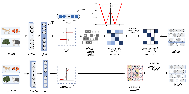
\includegraphics[width=0.95\linewidth]{papers_img/comparision_D2H_final.pdf}
    \caption{Comparison between deep learning for hashing and classification.}
    \label{Fig:comparison_classification_vs_hash}
        \vspace{-3ex}
\end{figure}
